\documentclass[aspectratio=169, 10pt, shadow]{beamer}

% --- 1. VISUAL CONFIGURATION (FEUP STYLE) ---
\usetheme{Madrid}
\usecolortheme{beaver} 

% Custom FEUP Red Colors
\definecolor{FEUPRed}{RGB}{140, 0, 0}
\setbeamercolor{structure}{fg=FEUPRed}
\setbeamercolor{frametitle}{bg=FEUPRed!10!white, fg=FEUPRed}
\setbeamercolor{block title}{bg=FEUPRed, fg=white}
\setbeamercolor{block body}{bg=FEUPRed!5!white, fg=black}

\usefonttheme{serif}
\usepackage{mathpazo} 
\usepackage[utf8]{inputenc}
\usepackage[english]{babel}
\usepackage{amsmath}
\usepackage{graphicx}
\usepackage{booktabs}
\usepackage{caption}

% Table of Contents Settings
\setbeamertemplate{section in toc}[ball unnumbered]
\setbeamertemplate{subsection in toc}[ball unnumbered]

\makeatletter
\patchcmd{\beamer@sectionintoc}{\vskip1.5em}{\vskip1.2em}{}{}
\patchcmd{\beamer@subsectionintoc}{\vskip1.5em}{\vskip0.4em}{}{}
\makeatother

% --- 2. PRESENTATION DATA ---
\title[SWAID Plate Resonance]{Resonance of a Chladni plate through a FPGA and a RaspberryPI}
\subtitle{Systems Engineering - Group 13}

\author[Group 13]{}

\institute[FEUP]{
  \textbf{Master in Electrical and Computer Engineering} \\
  Faculdade de Engenharia da Universidade do Porto \\
  \vspace{0.3cm}
  \textbf{Professor:} Sérgio Reis Cunha
}
\date{\today}
\titlegraphic{
\includegraphics[width=0.18\linewidth]{images/feup_logo.jpg}} 

\begin{document}

% --- SLIDE 1: COVER ---
\begin{frame}[plain]
  \titlepage
\end{frame}

% --- SLIDE 2: AGENDA ---
\begin{frame}{Agenda}
  \begin{columns}[t]
    \column{0.02\textwidth} 
    \column{0.96\textwidth}
      \begin{itemize}
          \item[] \scriptsize \tableofcontents 
      \end{itemize}
  \end{columns}
\end{frame}

% --- SECTION 1: PROPOSAL/CHALLENGE ---
\section{Proposal \& Challenge}
\begin{frame}{Challenge Definition}
  \begin{block}{Instructions}
    Define the core functions and capabilities the system must possess. Focus on identifying initial interfaces and dependencies between the FPGA, the Raspberry Pi, and the mechanical plate.
  \end{block}
  \begin{itemize}
      \item Describe the problem: Visualizing acoustic resonance.
      \item Evaluate initial constraints and external impacts (e.g., noise, power).
  \end{itemize}
\end{frame}

% --- SECTION 2: TEAM ---
\section{Team Structure}
\begin{frame}{Team Organization}
  \begin{columns}[t]
    \begin{column}{0.30\textwidth}
      \setbeamercolor{postit}{fg=black,bg=gray!10}
      \begin{beamercolorbox}[sep=0.8em, wd=\textwidth, rounded=true, shadow=true]{postit}
          \textbf{Members List}
          \small
          \begin{itemize}
              \item A. Cruz (up202204984) \item A. Gorra (up202207016)
              \item A. Kovbasa (up202208696) \item A. Vijayakumar (up202510629)
              \item B. Martins (up202108091) \item G. Bezerra (up202202477)
              \item H. Gomes (up202208777) \item J. Oliveira (up202205302)
              \item J. Pinto (up202207394) \item L. Aparício (up202206594)
              \item M. Amorim (up202208665)
          \end{itemize}
      \end{beamercolorbox}
    \end{column}
    \begin{column}{0.65\textwidth}
        \textbf{Instructions}
        \begin{itemize}
            \item Map the 11 roles to specific system functions.
            \item Define boundaries for each department (Hardware vs. Software) to reduce integration risks.
        \end{itemize}
        \centering
        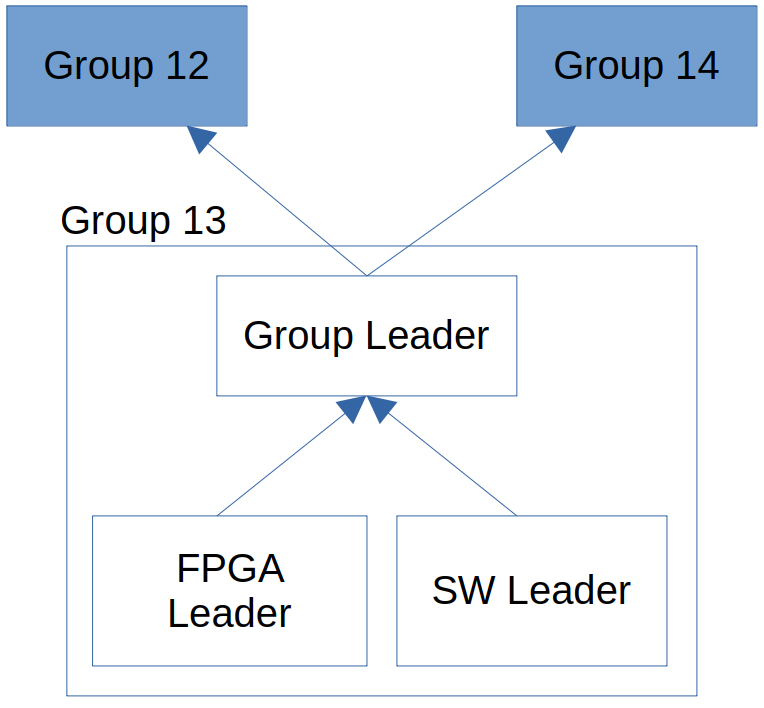
\includegraphics[width=0.5\linewidth]{images/team_structure.png}
    \end{column}
  \end{columns}
\end{frame}

% --- SECTION 3: SYSTEM CONCEPT ---
\section{System Concept}
\subsection{Validated Requirements}
\begin{frame}{System Requirements}
  \begin{block}{Instructions}
    Determine the specific inputs and outputs required for each requirement. List the technical characteristics the system must maintain to achieve resonance.
  \end{block}
\end{frame}

\subsection{Verified Functional Architecture}
\begin{frame}{Functional Context}
  \centering
  \begin{itemize}
      \item Determine information flow between the UI and transducers/lights.
      \item Identify all interfaces and dependencies to ensure a clear system boundary.
  \end{itemize}
  %\includegraphics[width=0.5\linewidth]{functional_arch.png}
\end{frame}

\subsection{System Baseline and SBS}
\begin{frame}{System Breakdown Structure (SBS)}
  \begin{block}{Instructions}
    Break down the system into hierarchies. This helps in understanding the set of functions each sub-level must possess to reduce integration risks.
  \end{block}
\end{frame}

\subsection{MOEs and MOPs}
\begin{frame}{Measures of Effectiveness (MOEs)}
  \begin{itemize}
      \item Quantify the "capabilities" identified in your functional context.
      \item How will you evaluate the constraints and external impacts on performance?
  \end{itemize}
\end{frame}

% --- SECTION 4: SYSTEM DESIGN ---
\section{System Design}
\subsection{Design Architecture Mapping}
\begin{frame}{Mapping Functional to Design Architecture}
  \begin{block}{Instructions}
    Show how the functions identified in the "Functional Context" map to specific hardware (FPGA) or software (Pi) components.
  \end{block}
\end{frame}

\subsection{Design Rationale}
\begin{frame}{Design Rationale (The "Why")}
  \begin{itemize}
      \item Why was this specific set of characteristics chosen?
      \item Explain how this design minimizes external impacts and constraints.
  \end{itemize}
\end{frame}

% --- SECTION 5: OUTCOME ---
\section{Outcome of the Project}
\subsection{What has been achieved}
\begin{frame}{Project Achievements}
  \begin{itemize}
      \item Summarize the final capabilities achieved by the system.
      \item Did the final flow of information match your initial functional context?
  \end{itemize}
\end{frame}

\subsection{Final Product}
\begin{frame}{Prototype Overview}
  \centering
  %\includegraphics[width=0.4\linewidth]{final_product.png}
  \begin{block}{Instructions}
    Present the physical manifestation of your functional boundaries.
  \end{block}
\end{frame}

\subsection{Tests}
\begin{frame}{Experimental Results}
  \begin{itemize}
      \item Present data showing that inputs correctly lead to expected outputs (nodal lines).
  \end{itemize}
\end{frame}

\subsection{Validation and Verification}
\begin{frame}{V\&V Results}
  \begin{itemize}
      \item Verification: Did the characteristics and capacities match the design?
      \item Validation: Does the system possess the functions the user actually needs?
  \end{itemize}
\end{frame}

\subsection{Cost Structure}
\begin{frame}{Financial Analysis}
  \begin{itemize}
      \item Evaluate the financial constraints and impacts on the project outcome.
  \end{itemize}
\end{frame}

% --- SECTION 6: MANAGEMENT ---
\section{Management Approach}
\subsection{Organization and Roles}
\begin{frame}{Roles and Responsibilities}
  \begin{itemize}
      \item Detail how defining clear boundaries helped in managing 11 team members.
  \end{itemize}
\end{frame}

\subsection{Conflict Management}
\begin{frame}{Conflict Resolution}
  \begin{itemize}
      \item Describe how you managed constraints regarding internal team dynamics.
  \end{itemize}
\end{frame}

\subsection{WBS + Gantt}
\begin{frame}{Project Timeline}
  \centering
  %\includegraphics[width=0.6\linewidth]{gantt.png}
\end{frame}

\subsection{Risk Management}
\begin{frame}{Risk Analysis}
  \begin{itemize}
      \item How did you reduce integration risks with other systems?
      \item Evaluate external impacts that could have delayed the project.
  \end{itemize}
\end{frame}

% --- SECTION 7: CONCLUSIONS ---
\section{Lessons Learned}
\begin{frame}{Observations}
  \begin{itemize}
      \item Reflect on the ease or difficulty of defining clear functional boundaries.
  \end{itemize}
\end{frame}

\section{Final Evaluation}
\begin{frame}{Internal Review}
  \begin{itemize}
      \item Self-assessment based on the project objectives.
  \end{itemize}
\end{frame}

% --- FINAL SLIDE ---
{
\usebackgroundtemplate{}
\begin{frame}[plain]
  \centering
  \vspace{1.5cm}
  {\Huge \textcolor{FEUPRed}{\textbf{Thank you for your attention!}}} \\
  \vspace{1cm}
  
\includegraphics[width=0.15\linewidth]{images/feup_logo.jpg}
\end{frame}
}

\end{document}